% Построение аппроксимаций данных, полученных при компьютерном моделировании притока жидкости к вертикальной скважине (пдф/пкв)

\chapter{Исследование данных до обучения моделей} \label{ch1}
В первой главе будет исследован характер данных в обоих рассматриваемых датасетах, для которых в дальнейшем будут строиться аппроксимации.
\section{Тепловая карта корреляций} \label{ch1:sec1}
Построим тепловую карту корреляций (рис. \ref{fig:heat-map-1}) между входными и выходными параметрами первого датасета (сценарий 1).

\begin{figure}[H] 
	\center
	\includegraphics[width=\textwidth]{images/corr_matrix_scenario1}
	\caption{Тепловая карта корреляций (сценарий 1)} 
	\label{fig:heat-map-1}
\end{figure}
Из построенной карты корреляций видим, что есть сильная линейная корреляция между соседними значениями дебитов, что может быть теоретически использовано для воспроизведения полной последовательности значений дебитов в том случае, когда известны только несколько значений из этой последовательности. 

Более значимое для построения аппроксимаций наблюдение состоит в том, что в первые месяцы на значения дебитов нефти наиболее сильно влияют пористость и проницаемость трещин. После первого года влияние проницаемости трещин снижается и возрастает влияние проницаемости матрицы. После второго года снижается влияние проницаемости матрицы и возрастает влияние пористости матрицы и пористости трещин.

\begin{figure}[H] 
	\center
	\includegraphics[width=\textwidth]{images/corr_matrix_scenario2}
	\caption{Тепловая карта корреляций (сценарий 2)} 
	\label{fig:heat-map-2}
\end{figure}

Тепловая карта корреляций для второго сценария (рис. \ref{fig:heat-map-2}) в первый год сильно отличается от первого сценария, так как во втором сценарии сначала рассматривается другой режим работы (естественный режим) и только затем включается нагнетание. Также во втором сценарии появляется заметная отрицательная корреляция между выходными дебитами, что тоже связано с запаздыванием включения системы ППД по сравнению с первым сценарием.

\section{Распределения выходных параметров} \label{ch1:sec2}
Построим распределения выходных параметров для того, чтобы проанализировать, каким образом изменялось распределение возможных значений выходных параметров с течением времени. Для первого сценария разработки (рис. \ref{fig:histograms-1}) видим, что большинство значений дебитов в первый месяц сосредоточены в области более низких значений, затем при переходе к концу первого года большинство возможных значений дебитов плавно переходит в область высоких значений. К концу пятого года разработки большинство значений сосредоточены в области средних значений.

\begin{figure}[H] 
	\center
	\includegraphics[width=\textwidth]{images/parameters_histograms_scenario1}
	\caption{Распределения нескольких выходных параметров (сценарий 1)} 
	\label{fig:histograms-1}
\end{figure}

Во втором сценарии (рис. \ref{fig:histograms-2}) в первый год разработки выражено разделение значений дебитов на кластеры, так как кейсы делятся на группы по критерию начала включения системы ППД. Далее характер распределений аналогичен первому сценарию.

\begin{figure}[H] 
	\center
	\includegraphics[width=\textwidth]{images/parameters_histograms_scenario2}
	\caption{Распределения нескольких выходных параметров (сценарий 2)} 
	\label{fig:histograms-2}
\end{figure}



\section{Диаграмма рассеяния} \label{ch1:sec3}
Диаграммы рассеяния позволяют наглядно проверить утверждения, полученные при анализе тепловых карт. Например, для первого сценария из тепловой карты видели, что наиболее существенный вклад в значения дебитов в первый месяц оказывают пористость и проницаемость трещин.
Построив диаграмму рассеяния (рис. \ref{fig:scatter-1}) для значений дебитов нефти в первый месяц и соответствующих значений проницаемости трещин (по оси абсцисс), пористости трещин (ранжирование значений с помощью цвета), видим, что замеченные ранее из тепловой карты линейные связи явно выделяются: на диаграмме линейный тренд и плавный переход по цветовой гамме.

Другими словами, видим, что возможно предсказать примерное значение дебита нефти в первый месяц из проницаемости и пористости трещин, а пористость и проницаемость матрицы оказывают незначительное влияние на это значение.
\begin{figure}[H] 
	\center
	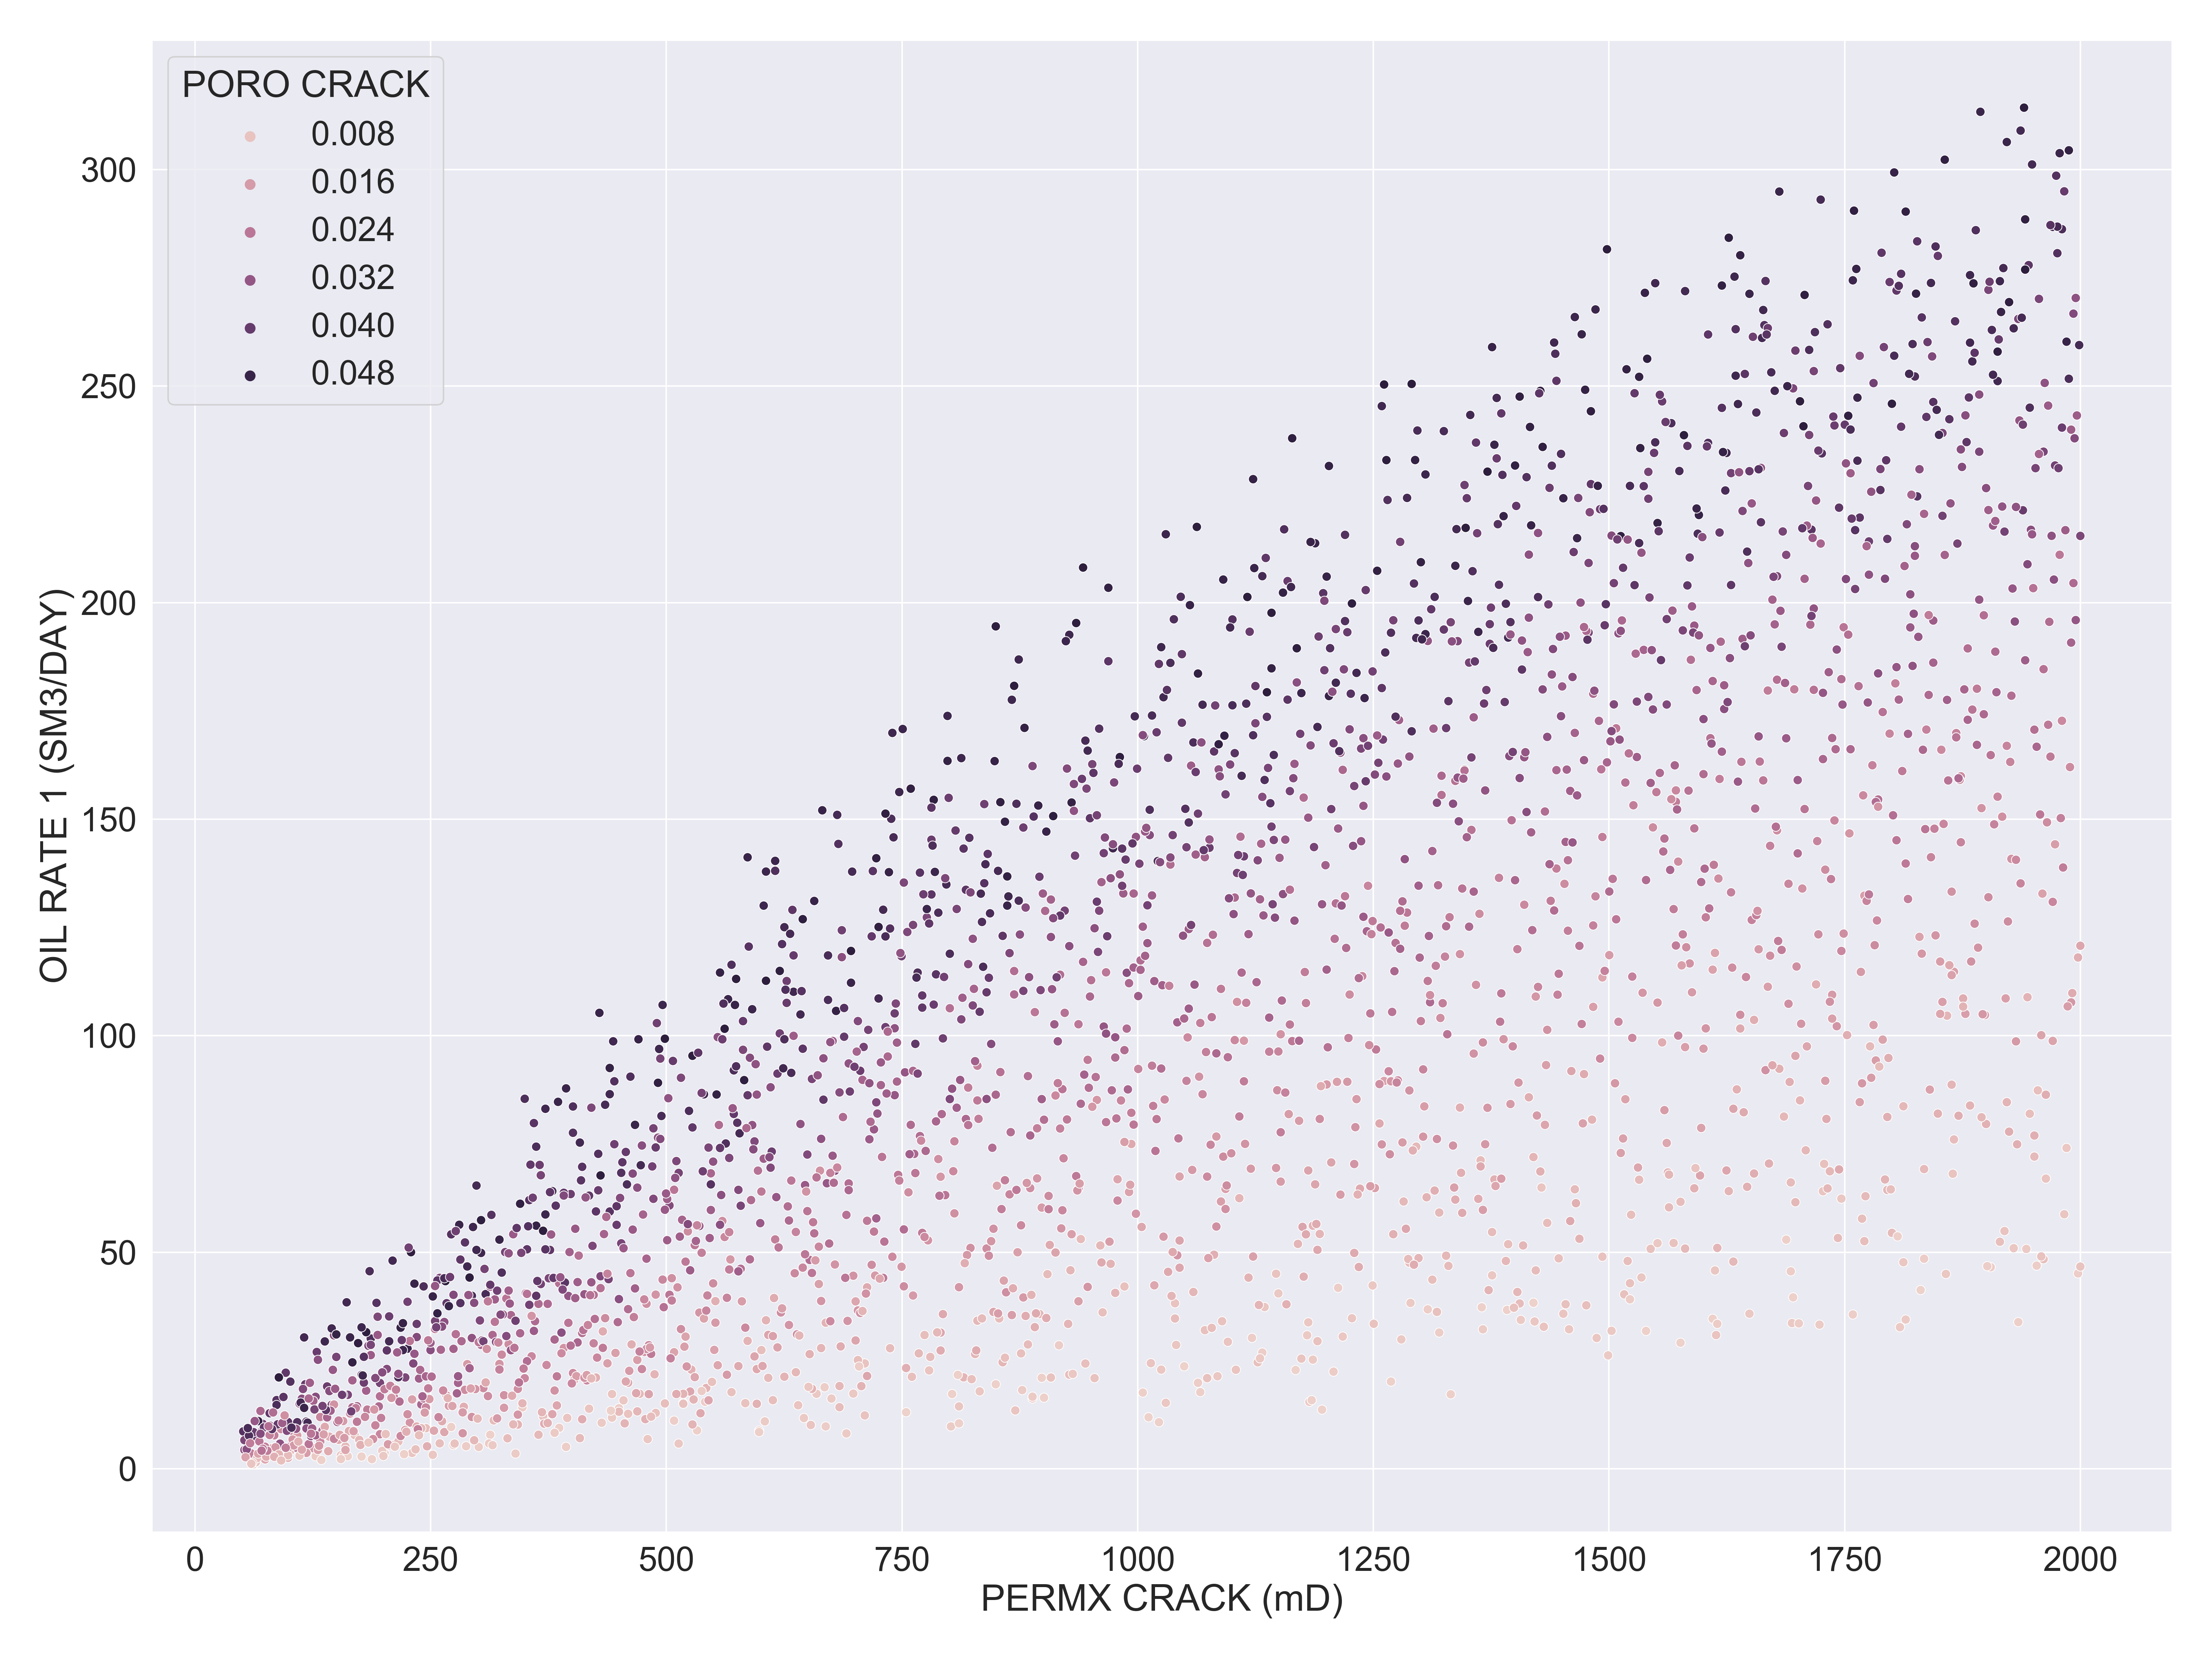
\includegraphics[width=\textwidth]{images/all_data_scatterplot_1}
	\caption{Диаграмма рассеяния, первый месяц (сценарий 1)} 
	\label{fig:scatter-1}
\end{figure}

Похожая диаграмма рассеяния имеет место быть для значений дебитов в последний месяц и соответствующих значений пористости матрицы и пористости трещин (рис. \ref{fig:scatter-2}), так как на тепловой карте (см. рис. \ref{fig:heat-map-1}) есть значительная линейная корреляция между значениями дебитов в последние месяцы и соответствующими пористостями матрицы и трещин.

\begin{figure}[H] 
	\center
	\includegraphics[width=\textwidth]{images/all_data_scatterplot_2}
	\caption{Диаграмма рассеяния, последний месяц (сценарий 1)} 
	\label{fig:scatter-2}
\end{figure}


\section{Выводы} \label{ch1:conclusion}

В результате исследования характера данных в рассматриваемых датасетах (сценарий 1, сценарий 2) для каждого месяца выделены наиболее влияющие на значения дебитов входные параметры. Также проведены визуализации, которые будут полезны для понимания результатов прогноза моделей машинного обучения. 

